\documentclass[border=2pt]{standalone}
\usepackage{pgfplots}
\pgfplotsset{compat=1.18}
\begin{document}
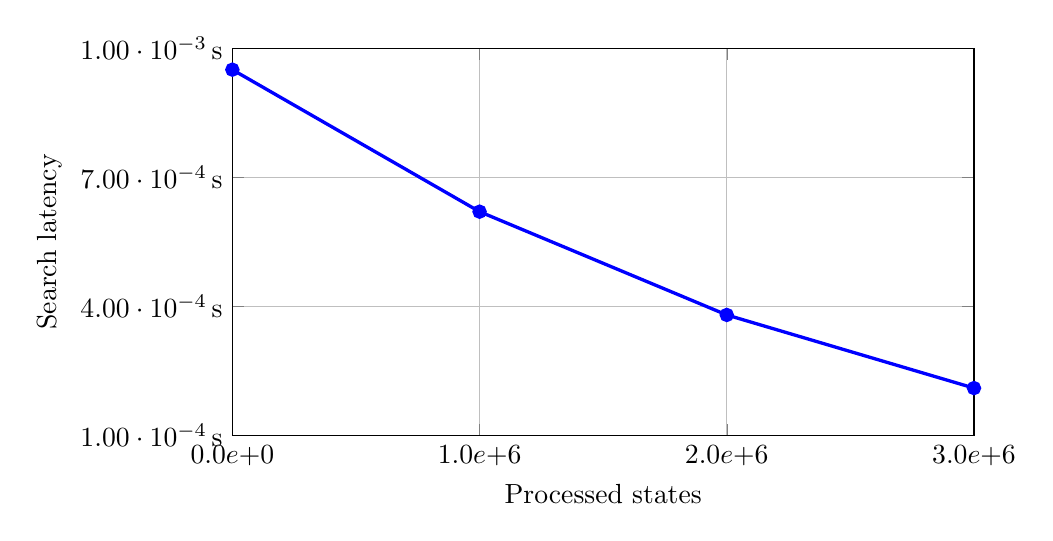
\begin{tikzpicture}
  \begin{axis}[
    width=11cm,
    height=6.5cm,
    xmin=0,
    xmax=3000000,
    ymin=0.0001,
    ymax=0.001,
    xtick={0,1000000,2000000,3000000},
    ytick={0.0001,0.0004,0.0007,0.001},
    scaled ticks=false,
    xticklabel={$\pgfmathprintnumber[sci,sci e,sci zerofill,precision=1]{\tick}$},
    yticklabel={$\pgfmathprintnumber[sci,sci 10^e,sci zerofill,precision=2]{\tick}\,\mathrm{s}$},
    grid=major,
    xlabel={Processed states},
    ylabel={Search latency}
  ]
    \addplot[blue,very thick,mark=*] coordinates {
      (0,0.00095) (1000000,0.00062) (2000000,0.00038) (3000000,0.00021)
    };
  \end{axis}
\end{tikzpicture}
\end{document}
